\subsection{Direct Fourier learning on a monotone graph}
\label{sec:direct_fourier_protocol}
This is the new protocol \path{direct_fourier_monotone_20261120_v1},
which supplies the current main Fourier learning and prediction evidence.
It is a nonlinear kinematic graph benchmark, not the earlier periodic dynamic
plant of Section~\ref{sec:normalized_fourier_results}. Its simulator uses
\begin{equation}
 y=.3+1.2x+.02\sin(20x),\qquad z=(x,y).
 \label{eq:df_graph}
\end{equation}
The formula and its physical row $F=(-1.2-.4\cos(20x),1)$ are used only by
the simulator and evaluator. The learner is given neither the residual
formula nor any physical coefficient, partial entry, or derivative target.
Both context units are fixed and dimensionless. It receives exact $x$ and
$\dot x$, noisy $\dot y_m=\dot y+\varepsilon_n$ with independent
$\varepsilon_n\sim\mathcal N(0,.0005^2)$, and known coordinate phase
$\phi=20x$. The phase and harmonic order $K=1$ are supplied representation
assumptions. Phase is derived from measured $x$, not an independently
manipulated physical input or an extra coordinate of $z$.

\paragraph{All-entry representation and coupled update.}
With $h=(1,\cos\phi,\sin\phi)^{\mathsf T}$, the unit row
$C\in\mathbb R^{1\times6}$ represents
\begin{align}
 \widehat H_C(x)&=C(h\otimes I_2),&
 w&=h\otimes(\dot x,\dot y_m)^{\mathsf T},\label{eq:df_lift}\\
 \dot R&=ww^{\mathsf T}-R/30,&
 \dot C&=-100\{CR-(CRC^{\mathsf T})C\}.
 \label{eq:df_update}
\end{align}
Every one of the six harmonic weights is independently adaptive, including
all three weights of the output entry. No potential is fitted and then
differentiated. Six independent standard-normal draws are normalized to
initialize $C$, without rejection or physical information; $R(0)=0$.
The initial $x_0$ is then drawn uniformly over one phase cycle. Seeds 10--19
vary these initializations and the sensor noise. The same-stream $K=0$
comparison learns a direct two-entry row from the identical measured
velocities, with the same gain, memory, and sample interval; its initial row
is the normalized first two entries of the $K=1$ initialization. This is an
ablation of the harmonic representation under matched settings, not a
comparison with an independently optimized alternative estimator.

Sampling is $\Delta t=.02$~s. Each observed $w_n$ is scored with the pre-update
row. Over its subsequent held-sample interval, the covariance is evaluated as
\begin{equation}
 R(s)=e^{-s/30}R_n+30(1-e^{-s/30})w_nw_n^{\mathsf T}.
 \label{eq:df_memory}
\end{equation}
DOP853 integrates $\dot a=-100R(s)a$, starting at $a(0)=C_n^{\mathsf T}$,
with relative and absolute tolerances $10^{-9}$ and $10^{-11}$; the returned
row is $a^{\mathsf T}/\|a\|$. Thus memory evolves within each integration
step. This implements the coupled normalized law, not a frozen-memory
exponential or an instantaneous bottom-eigenvector update. All coefficient
and covariance states before each observation are saved.

Training imposes coefficient normalization only; no all-phase row-norm
constraint is enforced. This is the unguarded normalized flow, not a feasible
projection onto the main paper's phase-constrained set. A postprocessing check
of saved states makes the distinction concrete: for seed 11 at $t=5.06$ s,
the learned field has norm $5.37\times10^{-5}$ at phase $-.675677$.
Thus a $.05$ all-phase row-norm bound would fail at that training state.
No prediction task uses these intermediate fields. Readout feasibility is
checked separately for the final frozen field below; the diagnostic and its
saved-state identity are retained in \path{row_norm_guard_diagnostic.json}.


\paragraph{Actual input and partial timescales.}
The training input over $0\le t\le240$~s is
\begin{equation}
 x=x_0+.15t+.05\sin(.3t),\qquad
 \dot x=.15+.015\cos(.3t).
 \label{eq:df_train_input}
\end{equation}
The actual supplied coordinate is a monotone ramp plus slow modulation;
its actual rate modulates at $.3$~rad/s. Physical partial variation follows
$\dot\phi=20\dot x\in[2.7,3.3]$~rad/s, nine to eleven times that modulation.
This comparison uses the executed input, not merely a desired reference.
The output rate $\dot y$ is fast and is not called a slow input.
For seed~10, the empirical derivative-RMS/centered-RMS rate scales are
$.01447$ for $x$, $.30100$ for $\dot x$, $3.00995$ for the physical slope,
and $2.91343$ for $\dot y$, in inverse seconds. The statistic for the ramp
$x$ depends on the observation duration and is not a stationary spectral
frequency. These diagnostics do not claim that every learner channel is slow.

\paragraph{Independent prediction using the same learned field.}
At 240~s learning stops. A new 30-s episode uses
\begin{align}
 x(t)&=x_{\rm final}+.12t+\frac{.03}{.47}(1-\cos(.47t)),\\
 \dot x(t)&=.12+.03\sin(.47t),\qquad 0\le t\le30~\mathrm{s}.
 \label{eq:df_test_input}
\end{align}
Its actual rate modulation is $.47$~rad/s, while the physical partial phase
rate lies in $[1.8,3.0]$~rad/s. With $C$ frozen, the original learned field
computes
\begin{equation}
 \widehat{\dot y}=-\widehat H_x\dot x/\widehat H_y.
 \label{eq:df_readout}
\end{equation}
The predicted output is integrated by the trapezoidal rule from one measured,
exact initial $y$. No later $y$ or $\dot y$ is supplied to the readout or
assimilated into the prediction. Supplied $x$ follows the prescribed actuator
motion, so it is not a hidden future output. Each seed learns on one
continuous training trajectory; the subsequent episode tests prediction and
is not an additional perturbation trial used for identification.

A query with $|\widehat H_y|<.05$ is invalid, with no oracle fallback.
Writing the output weights as $(C_{01},C_{11},C_{21})$ gives the elementary
all-phase bound
\begin{equation}
 |\widehat H_y|\ge |C_{01}|-\sqrt{C_{11}^2+C_{21}^2}.
 \label{eq:df_guard}
\end{equation}
The minimum final bound across all ten seeds is $.6195546$, and all 15,010
learned heldout queries pass the guard. This is a final frozen-model bound,
not a continuous-time guarantee during training: 376 recorded training
snapshots would fail the query guard, when no prediction task was requested.
The frozen initial $K=1$ prior has 916 invalid heldout queries in seven runs;
its full-episode errors are recorded as undefined in those cases, not
replaced by selected valid-query averages. The $K=0$ heldout queries have
no guard failures.

\paragraph{Separate learning, recovery, and task evidence.}
The physical row is evaluator-only. At each observed context, the record
contains $\tfrac12(\widehat H_C\dot z_m)^2$, the Frobenius difference between
the estimated and physical row projectors, and the separately scored task
errors. Row normalization/sign alignment is used only for display and never
changes the field used for a query. On $[200,240)$~s, the ten-seed mean
row-projector error is $(6.3912\pm1.3368)10^{-5}$, versus
$.150378\pm.000704$ for $K=0$. Mean observed pre-update energy is
$(4.8266\pm.1652)10^{-8}$, versus
$(3.66434\pm.01684)10^{-4}$ for $K=0$.
Prediction rate RMSE is $(1.60965\pm.46632)10^{-5}$ and integrated-output
RMSE is $(9.24323\pm6.70758)10^{-5}$. Corresponding $K=0$ errors are
$.0354751\pm.0001978$ and $.100628\pm.015898$.
All $\pm$ values denote sample standard deviations across the ten specified
seeds. Table~\ref{tab:direct_fourier_all_seeds} preserves every seed.

\begin{table*}[t]
\centering
\caption{New direct Fourier benchmark, all prespecified seeds. Projector
error is the mean on $[200,240)$~s; rate and output RMSE use the independent
30-s episode. Scaled columns indicate their multipliers in the headings.
The last column counts invalid queries of the frozen initial $K=1$ prior;
the trained $K=1$ and $K=0$ predictors have none.}
\label{tab:direct_fourier_all_seeds}
\begin{tabular}{rrrrrrr}
\toprule
Seed & \shortstack{Projector\\($10^{-5}$)} & \shortstack{Rate RMSE\\($10^{-5}$)} & \shortstack{Output RMSE\\($10^{-5}$)}
& \shortstack{$K=0$\\rate RMSE} & \shortstack{$K=0$\\output RMSE} & \shortstack{Prior\\invalid}\\
\midrule
10 & 5.9683 & 1.7412 & 12.5246 & 0.035598 & 0.109743 & 0\\
11 & 4.7770 & 1.4933 & 6.6561 & 0.034956 & 0.062450 & 0\\
12 & 7.7329 & 1.4550 & 5.0253 & 0.035570 & 0.110815 & 126\\
13 & 7.0664 & 1.9766 & 18.0278 & 0.035479 & 0.112136 & 0\\
14 & 5.3648 & 2.0516 & 22.4932 & 0.035639 & 0.102372 & 60\\
15 & 6.8780 & 1.6651 & 2.7531 & 0.035492 & 0.099707 & 256\\
16 & 5.4824 & 0.9637 & 3.2382 & 0.035392 & 0.085399 & 133\\
17 & 7.6658 & 2.0401 & 3.5015 & 0.035477 & 0.112295 & 101\\
18 & 8.3966 & 2.0018 & 10.8025 & 0.035527 & 0.111805 & 159\\
19 & 4.5798 & 0.7081 & 7.4099 & 0.035622 & 0.099562 & 81\\

\bottomrule
\end{tabular}
\end{table*}

\begin{figure*}[t]
\centering
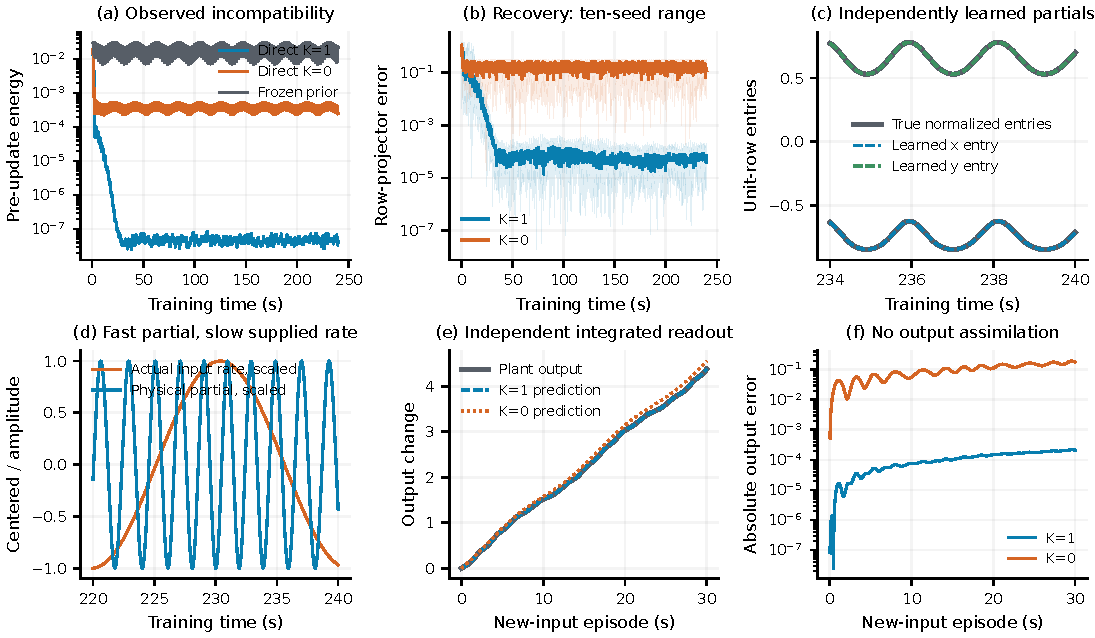
\includegraphics[width=.98\textwidth]{direct_fourier_summary.pdf}
\caption{Current direct Fourier evidence. Panels (a,c--f) use prospectively
selected seed~10; (b) shows the median and full range over all ten seeds.
Panel (a) is a causal 1-s mean of pre-update observed energy. Panel (c)
uses unit/sign alignment only for evaluating the two independently learned
entries. Panel (d) centers the actual input rate and physical partial and
divides each by its amplitude. Panels (e,f) integrate the same learned
readout on a new input, without later output assimilation.}
\label{fig:direct_fourier_new}
\end{figure*}

The final clean coefficient-covariance gap ranges from $.0054964$ to
$.0055467$, and $\|R_{\rm clean}C_*^{\mathsf T}\|$ is at most
$4.13\times10^{-15}$. Noisy covariance spectra and target-memory bias are
saved separately. A positive noisy eigengap is not treated as proof of
physical identification or unbiased recovery. All six coefficient entries
change in every run; the largest unit-norm error is $3.34\times10^{-16}$.
The generic learned field need not itself be a Jacobian. In this graph
geometry, wherever $\widehat H_y\ne0$, the gauge-equivalent field
$\widehat H/\widehat H_y=(\widehat H_x/\widehat H_y,1)$ is the gradient of
$y+\int (\widehat H_x/\widehat H_y)\,dx$. This post hoc interpretation does
not supply a potential to training and does not establish general
high-dimensional integrability.

\paragraph{Prespecification, verification, and provenance.}
The protocol fixed seeds 10--19, illustration seed~10, durations, observations,
initialization, baselines, and criteria before any new run. The excluded
exploratory pilot uses seed~9001. Each confirmatory seed passes the declared
limits: late mean projector error below $.01$, heldout rate RMSE below
$.002$, output RMSE below $.02$, and no learned heldout guard failure. These
are numerical evidence thresholds, not theorem hypotheses or significance
tests. No heldout result was used for tuning, and no run was omitted.

Two predeclared noise-free seed-10 refinements use $\Delta t=.02$ and $.01$~s.
Their final coefficient rows differ by at most $1.15\times10^{-14}$;
rate errors are below $1.84\times10^{-15}$ and integrated-output RMSE decreases
from $4.37321\times10^{-6}$ to $1.09337\times10^{-6}$. Direct projector
subtraction gives late errors below $10^{-14}$. The original equivalent
$\sqrt{2(1-\cos^2\theta)}$ summaries suffer cancellation at this scale and
report about $4\times10^{-9}$; those immutable summaries and the diagnosed
discrepancy are retained. This arithmetic floor is not interpreted as a
physical recovery error. The clean check isolates quadrature and update
accuracy, not a robustness test for noisy derivative estimation.

An independent audit reconstructs every recorded covariance transition,
observation/RNG stream, heldout rate and integrated trajectory. Selected
updates are checked against a tighter direct integration of the full
nonlinear coupled $(C,R)$ equations. All thirteen cases---the ten
confirmatory seeds, pilot, and two refinements---pass. The evaluator slope
is separately checked by finite differences of the simulator graph.
The portable source and commands are under
\path{experiments/direct_submission/fourier/}: \path{run.py},
\path{protocol.json}, \path{audit.py}, \path{summarize_plot.py}, and
\path{REPRODUCE.txt}. Each raw run retains source, configuration, complete
observed rates and pre-update coefficient/covariance states, predictions,
evaluator-only channels, RNG states, environment, and SHA-256 manifest.
The raw evidence archive is identified separately by the accompanying package manifest;
a local package does not imply that it has already been published.
The benchmark supports direct field learning and independent prediction
under known phase/order and the stated sensors. It does not validate the
old periodic plant's control, unknown-frequency discovery, noisy-rate
estimation from position-only sensors, or global stability.
